\section{Preliminaries}



\subsection{Definitions}

\cpar{Native Multimodal Models (NMMs):}
Models that are trained from scratch on all modalities simultaneously without
relying on pre-trained LLMs or vision encoders. Our focus is on the
representative image and text modalities, where the model processes both text
and images as input and generates text as output.

\cpar{Early fusion:} Enabling multimodal interaction from the beginning, using
almost no modality-specific parameters (\eg, except a linear layer to patchify
images). Using a single transformer model, this approach processes raw
multimodal \edit{input—tokenized text and continuous image patches—with no
image discretization.} \edit{We} refer to the main transformer as
the decoder.

\cpar{Late fusion:} Delaying the multimodal interaction \edit{to} deeper layers,
typically after separate unimodal components \edit{has processed} each modality
independently (\eg, a vision encoder connected to an LLM).

\cpar{Modality-agnostic routing:} In sparse mixture-of-experts, \edit{modality-agnostic} routing
refers to relying on a learned router module that is trained jointly with the
model.

\cpar{Modality-aware routing:} Routing based on pre-defined rules such as
routing based on the modality type (\eg, vision-tokens, token-tokens).

\begin{table}[t!]
    \centering
    \setlength{\tabcolsep}{8pt}
    \renewcommand{\arraystretch}{1.0}
    \resizebox{1\linewidth}{!}{
    \begin{tabular}{c p{0.999\linewidth}}
         Expression & Definition  \\
         \shline
         \textbf{$N$}     & \normalfont{{Number of parameters in the multimodal decoder. For MoEs this refers to the \edit{active parameters.}}} \\
         \grayrow
         \textbf{$D$}     & \normalfont{{Total number of multimodal tokens.}} \\
         \textbf{$N_{v}$} & \normalfont{{Number of vision-only tokens.}} \\
         \grayrow
         \textbf{$D_{v}$} & \normalfont{{Number of parameters in the vision-specific encoder. Only exists in late-fusion architectures.}} \\
         \textbf{$C$}     & \small{{Total number of FLOPs, estimated as $C=6ND$ for early-fusion and $C=6(N_vD_v+ND)$ for late-fusion.}} \\
         \grayrow
         \textbf{$L$}     & \normalfont{{Average validation loss on interleaved image-text, image-caption, and text-only data mixtures.}} \\
    \end{tabular}}
    \caption{Definitions of the expressions used throughout the paper.}
    \label{tab:my_label}
\end{table}




\subsection{Scaling Laws}
We aim to understand the scaling properties of NMMs and how different
architectural choices influence trade-offs. To this end, we analyze our models
within the scaling laws framework proposed by~\citet{kaplan2020scaling,
hoffmann2022training}.
We compute FLOPs based on the total number of parameters, using the
approximation \(C = 6ND\), as adopted in prior
work~\citep{hoffmann2022training,abnar2025parameters}. However, we modify this
estimation to suit our setup: for late-fusion models, FLOPs is computed as
\(6(N_vD_v + ND)\).
We consider a setup where, given a compute budget \(C\), our goal is to predict
the model’s final \edit{loss}, as well as determine the optimal number of
parameters \edit{and} number of training tokens. Consistent with prior studies on LLM
scaling~\citep{hoffmann2022training}, we assume a power-law relationship between
the final model loss and both model size (\(N\)) and training tokens (\(D\)):




\begin{equation}
\label{eq:scaling_laws}
    L = E + \frac{A}{N^{\alpha}} + \frac{B}{D^{\beta}}.
\end{equation}



\noindent Here, \(E\) represents the lowest achievable loss on the dataset,
while \(\frac{A}{N^{\alpha}}\) captures the effect of increasing the number of
parameters, where a larger model leads to lower loss, with the rate of
improvement governed by \(\alpha\). Similarly, \(\frac{B}{D^{\beta}}\) accounts
for the benefits of a higher number of tokens, with \(\beta\) determining the
rate of improvement. Additionally, we assume a linear relationship between
compute budget (FLOPs) and both \(N\) and \(D\) (\(C \propto ND\)). This further
leads to power-law relationships detailed in \cref{tab:power_laws}.



\begin{figure}[t!]
    \centering
    \captionsetup{type=figure}
    \begin{subfigure}[t]{0.48\linewidth}
        \centering
        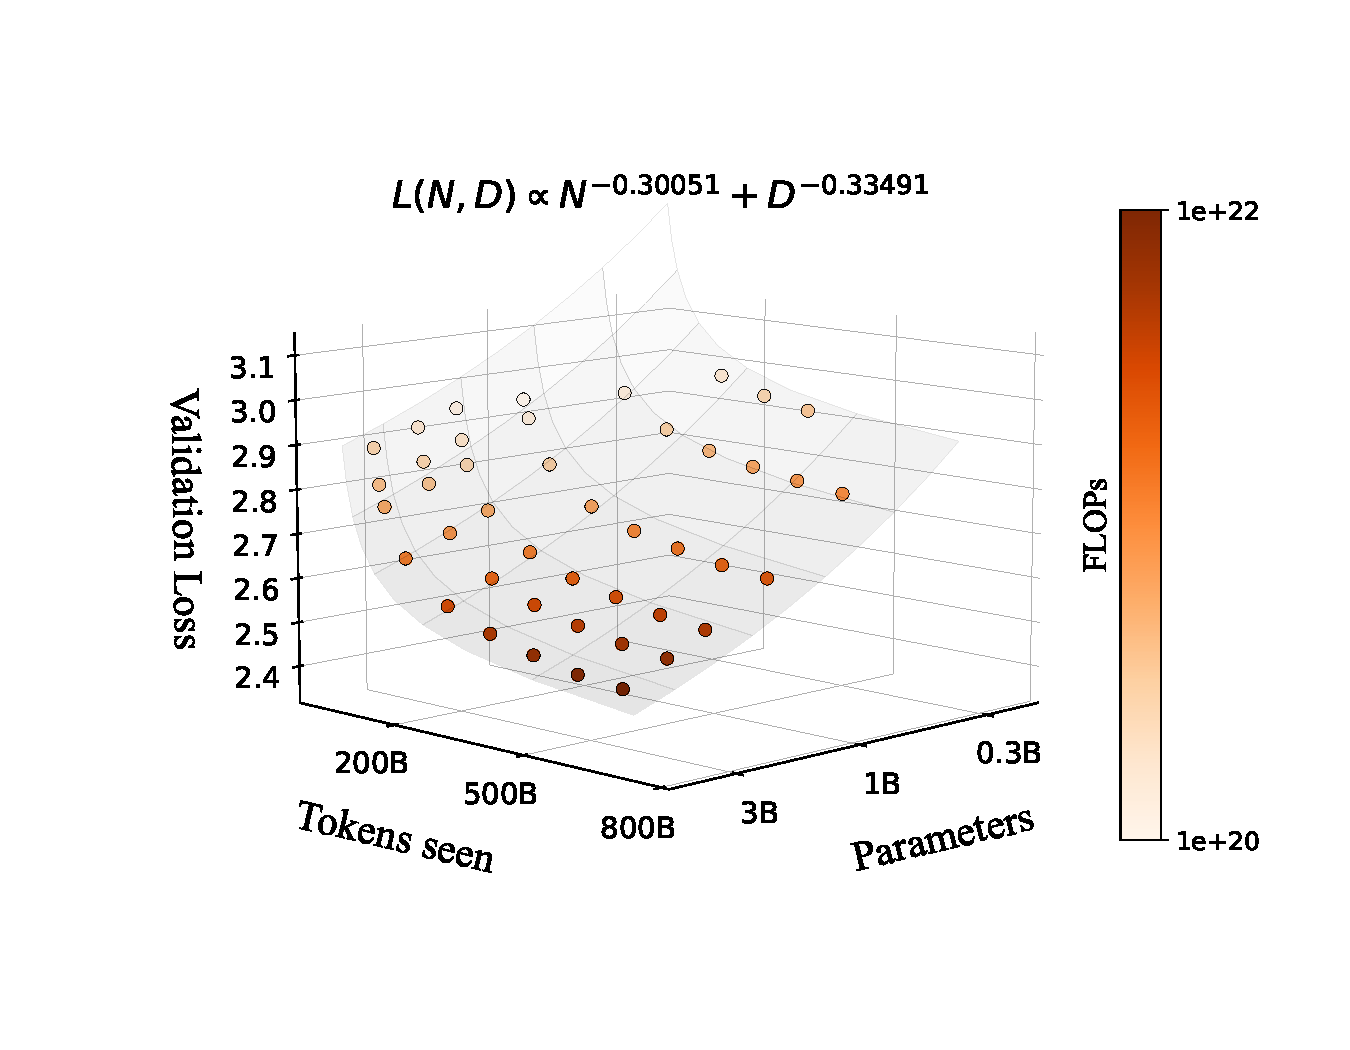
\includegraphics[width=1.02\linewidth]{assets/early/3d_scaling_early.pdf}
    \end{subfigure}
    \hfil
    \begin{subfigure}[t]{0.48\linewidth}
        \centering
        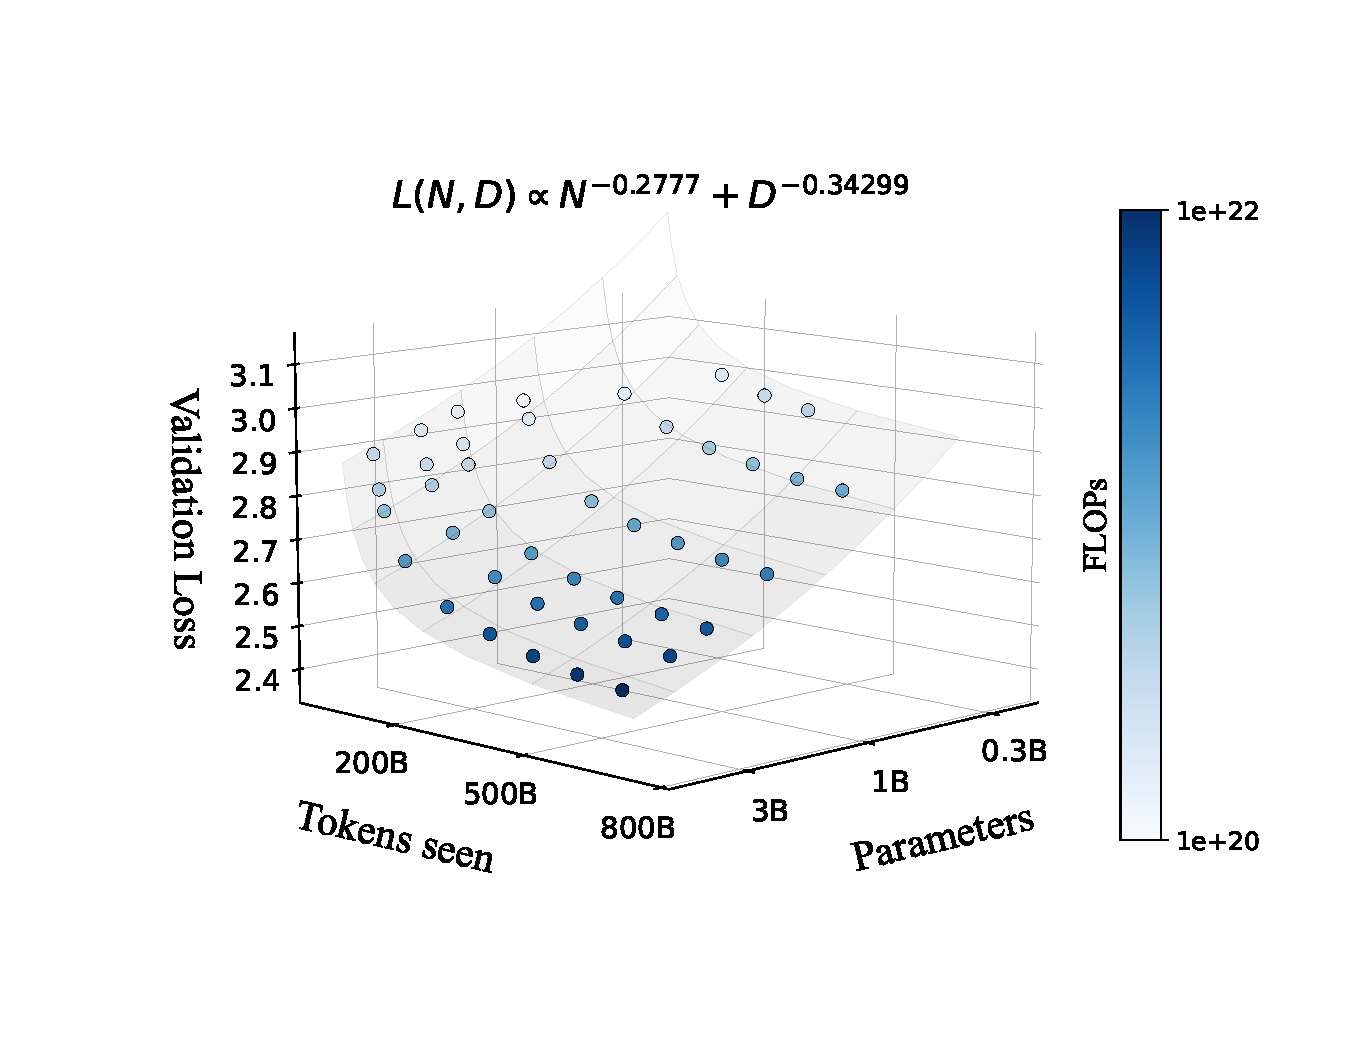
\includegraphics[width=1.02\linewidth]{assets/early/3d_scaling_late.pdf}
    \end{subfigure}
    \vspace{5pt}
    \setlength{\fboxsep}{0.5pt}
    \setlength{\fboxrule}{0pt}
    \caption{\textbf{Scaling laws for \fbox{\colorbox{CustomC_Light1!20}{\strut
    early-fusion}} and \fbox{\colorbox{CustomD_Light1!20}{late-fusion\strut}}
    native multimodal models.} Each point represents a model (300M to 3B
    parameters) trained on varying \edit{number of} tokens (250M to 400B). We
    report the average cross-entropy loss on the validation sets of
    \edit{interleaved (Obelics), Image-caption (HQITP), and text-only data
    (DCLM).}}
    \label{fig:early_vs_late_scaleflops_3d}
\end{figure}
        

\begin{table}[h]
    \centering
    \setlength{\tabcolsep}{16pt}
    \renewcommand{\arraystretch}{1}
    \resizebox{1\linewidth}{!}{
    \begin{tabular}{lccrc}
        Data type & dataset & \#samples & sampling prob. \\
         \shline
         \multirow{3}{*}{Image-Caption} &  DFN~\citep{fang2023data} & 2B & 27\%
         \\
          & COYO~{\citep{kakaobrain2022coyo700m}} &  600M & 11.25\% \\
          & HQITP  & 400M & 6.75\% \\
          Interleaved & Obelics \citep{laurenccon2024obelics}  & 141M Docs &
          45\% \\
          Text & DCLM \citep{li2024datacomp} & 6.6T Toks & 10\% \\
          
    \end{tabular}} \caption{\textbf{Pre-training data mixture.} Unless otherwise
    specified, the training mixture contains 45\%, 45\% and 10\% of image
    captions, interleaved documents and text-only data.}
    \label{tab:pretraining_datasets}
    \vspace{-5pt}
\end{table}

\subsection{Experimental setup}
\edit{Our models} are based on the autoregressive transformer
architecture~\citep{vaswani2017attention} with SwiGLU
FFNs~\citep{shazeer2020glu} and QK-Norm~\citep{dehghani2023scaling}
following~\citet{li2024datacomp}. In early-fusion models, image patches are
linearly projected to match the text token dimension, while late-fusion follows
the CLIP architecture~\citep{radford2021learning}. We adopt causal attention for
text tokens and bidirectional attention for image tokens, we found this to work
better. Training is conducted on a mixture of public and private multimodal
datasets, including DCLM \citep{li2024datacomp}, Obelics
\citep{laurenccon2024obelics}, DFN \citep{fang2023data}, COYO
\citep{kakaobrain2022coyo700m}, and a private collection of High-Quality
Image-Text Pairs (HQITP) (see \cref{tab:pretraining_datasets}). Images are
\edit{resized} to 224×224 resolution with a 14×14 patch size. We use a context
length of 1k for the multimodal sequences. For training efficiency, we train our
models with \texttt{bfloat16},  Fully Sharded Data Parallel (FSDP)
\citep{zhao2023pytorch}, \edit{activation} checkpointing, and gradient accumulation. We
also use sequence packing for the image captioning dataset to reduce the amount
of padded tokens. Similar to previous
works~\citep{hoffmann2022training,aghajanyan2023scalingmm,abnar2025parameters},
we evaluate performance on a held-out subsets of interleaved (Obelics),
Image-caption (HQITP), and text-only data (DCLM). Further implementation details
are provided in~\cref{app:implementation_details}.
